\documentclass[12pt,a4paper]{article}
\usepackage[utf8]{inputenc}
\usepackage[ngerman]{babel}
\usepackage[left=2.5cm,right=2.5cm,top=3cm,bottom=2cm]{geometry}
\author{Pauline Speckmann}
\usepackage{graphicx}
\usepackage{booktabs}

\usepackage{fancyhdr}
\pagestyle{fancy}
\fancyhf{}
\fancyhead[l]{Digitalisierung Vorlesung 5 $-$ Zusammenfassung von Pauline Speckmann}
\fancyhead[r]{\thepage}


\begin{document}

\setcounter{section}{4}
\section{Management der digitalen Transformation}


\vspace*{1cm}
\subsection{Transformationsstrategien entwickeln} %%%%%%%%%%%%%%%%%%%%%%%%%%%%%%%%%%%%%%%%%%%%%%%%%%%%%%%%%%%%%%%%%%%%%%%%%%%%%%%%%

\begin{itemize}
   \item \textbf{Sichten auf Transformationsstratiegien}

   \item[] $\rightarrow$ \textbf{Innovationsperspektive:}
      \begin{itemize}
         \item Phase 1: Experimentieren am Rande der Organisation
               \begin{itemize}
                  \item Ergänzende Experimente: \\
                        Das bestehende Geschäftsmodell bleibt bestehen, Innovation beruht auf das vorhandene Geschäftsmodell.
                  \item Disruptive Experimente: \\
                        Das Geschäftsmodell wird grundlegend innoviert.
                  \item Von der Beobachtung zur Verpflichtung:
                  \item[] 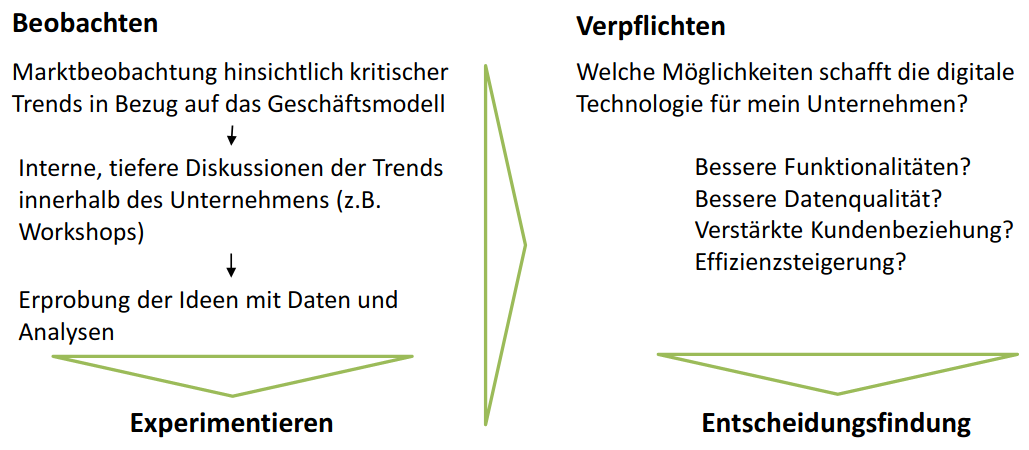
\includegraphics[scale=0.45]{experiment.png}
                  \item \emph{Black hole} vs. Optionen-orientierte Investment Strategien:
                  \item[] 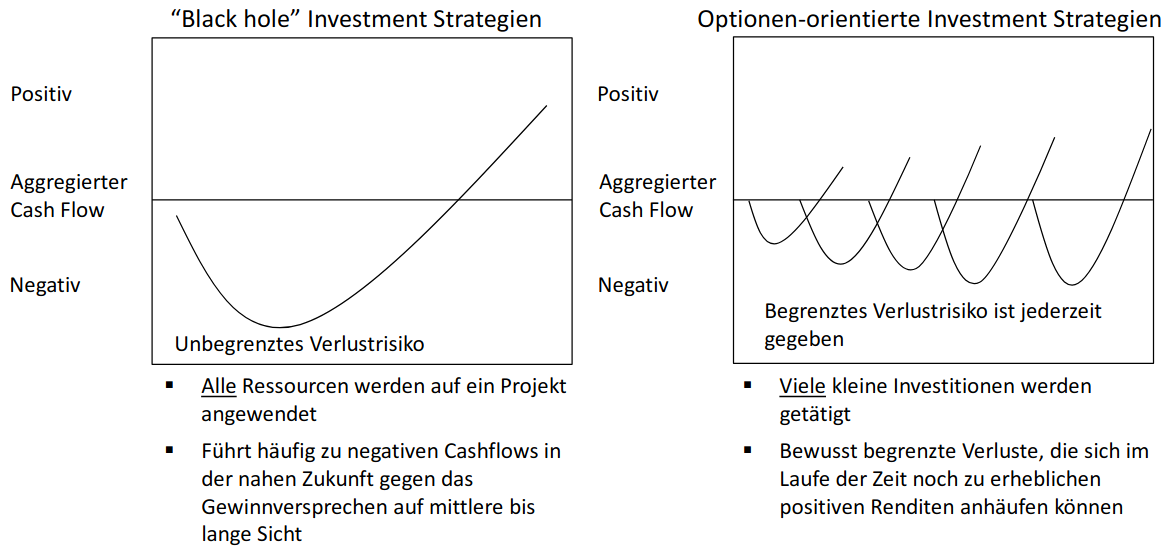
\includegraphics[scale=0.4]{bh.png}
               \end{itemize}

         \item Phase 2: Kollision im Kern (Alt/Traditionell vs. Neu/Modern)
               \begin{itemize}
                  \item Kollision von Strategien:\\
                        Aufstrebendes Start-Up vs. etabliertes Unternehmen der Branche vs. digitales Großunternehmen
                  \item Kollision der Organisation:\\
                        Effizienz-Nachteile in Durchlaufzeiten, Entscheidungsgeschwindigkeit, Führ\-ungs\-mo\-del\-le
                  \item Reaktionsebenen: Koexistenz vs. Morph\\
                        Wirksame und rechtzeitige Reaktion auf aufstrebende, digitale Konkurrenten.
                        \begin{itemize}
                           \item Ergänzung der Konkurrenten: Aufbau eines digitalen Geschäfts-modells als Koexistenz zum Konkurrenten
                           \item Morph: Ersetzen des traditionellen-durch ein digitales Geschäftsmodells
                        \end{itemize}
               \end{itemize}

         \item Phase 3: Neuerfindung an der Wurzel
               \begin{itemize}
                  \item Veränderung der Kernelemente des Geschäftsmodells durch digitale Technologien
               \end{itemize}

      \end{itemize}

   \item[] $\rightarrow$ \textbf{Architekturperspektive:}
      \begin{itemize}
         \item Geschwindigkeit  $\rightarrow$ hoher Innovationsgrad (viele Drittanbieter)
         \item Stabilität $\rightarrow$ zuverlässige Kernprozesse (enge Partner)
      \end{itemize}

   \item[] $\rightarrow$ \textbf{Führungsperspesktive:}
         \begin{itemize}
            \item[] 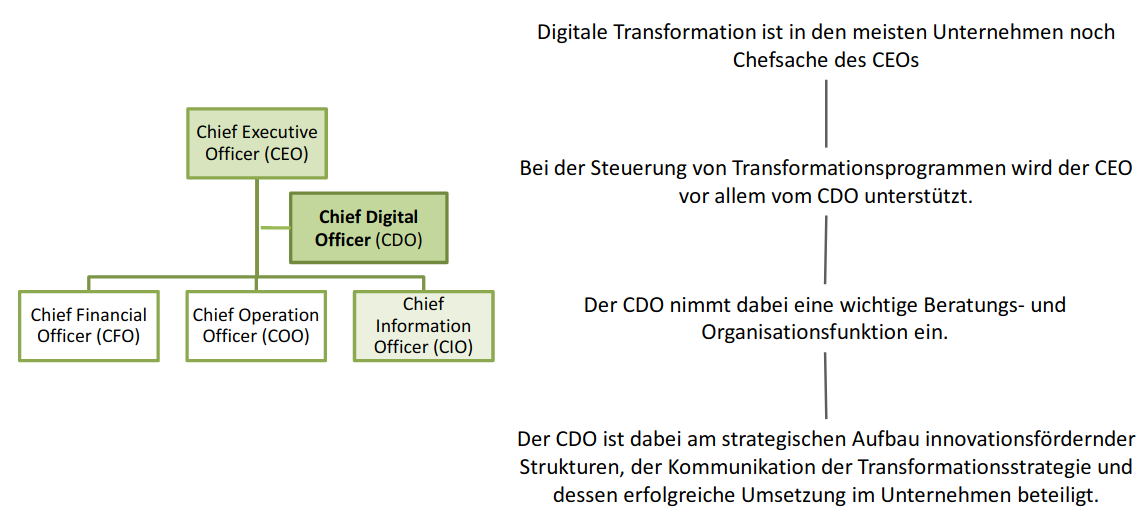
\includegraphics[scale=0.35]{ceo.png}
            \item CIO entwickelt IT-Strategie (IT-Expertenwissen)
            \item CDO legt fest (Digital-Strategisches Geschäftswissen)
            \item Unterschiede und Gemeinsamkeiten von CDO und CIO:
            \item[] 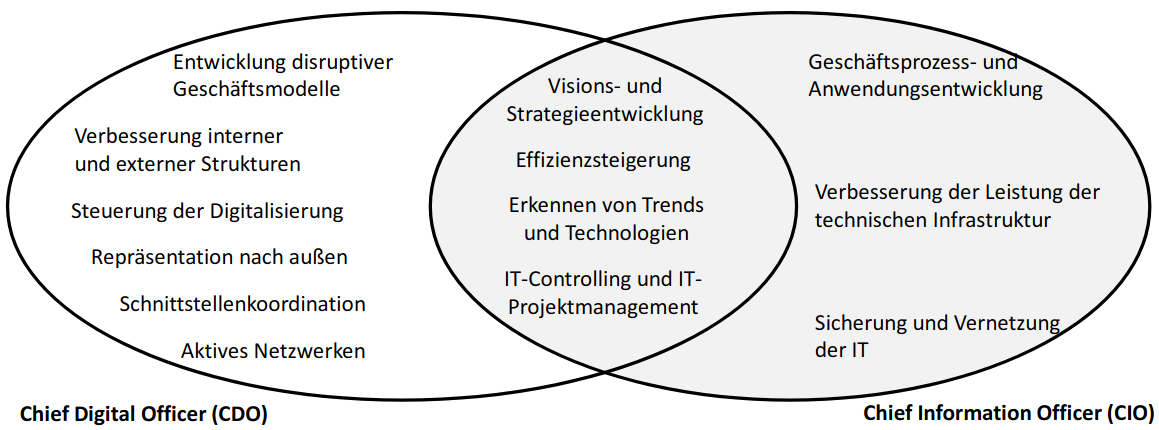
\includegraphics[scale=0.45]{ciocdo.png}
         \end{itemize}
         
\newpage %Manuelle Formatierung         
   \item \textbf{Entscheidungen einer Transformationsstrategie:}
   \item[] 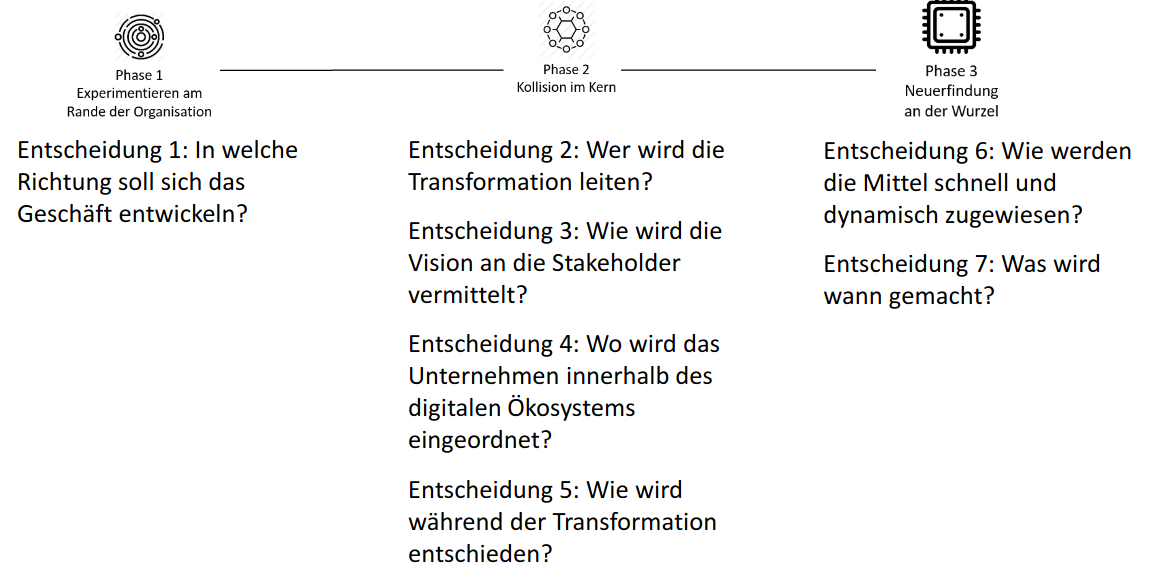
\includegraphics[scale=0.35]{dec.png}
\end{itemize}


\vspace{1cm}
\subsection{Voraussetzungen für die digitale Transformation schaffen} %%%%%%%%%%%%%%%%%%%%%%%%%%%%%%%%%%%%%%%%%%%%%%%%%%%%%%%%%%%%%%%%
\begin{itemize}
   \item \textbf{Die Acht Dimensionen der Digitalkultur:}
   \item[] 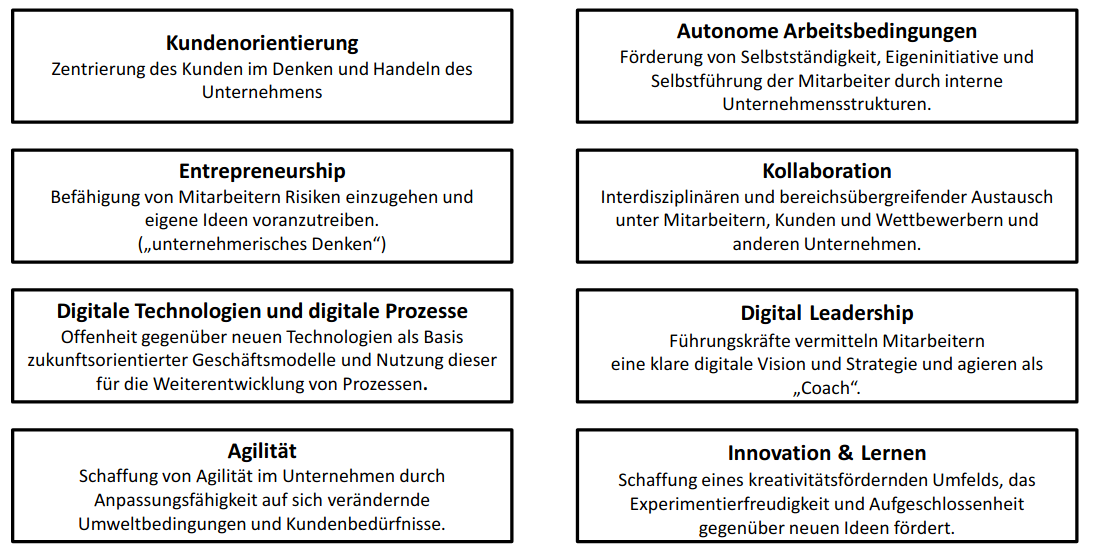
\includegraphics[scale=0.45]{8.png}
   
   \item \textbf{Transformationsfördernde OrganisationsstrukturenDigitalkultur:}
   \item[] 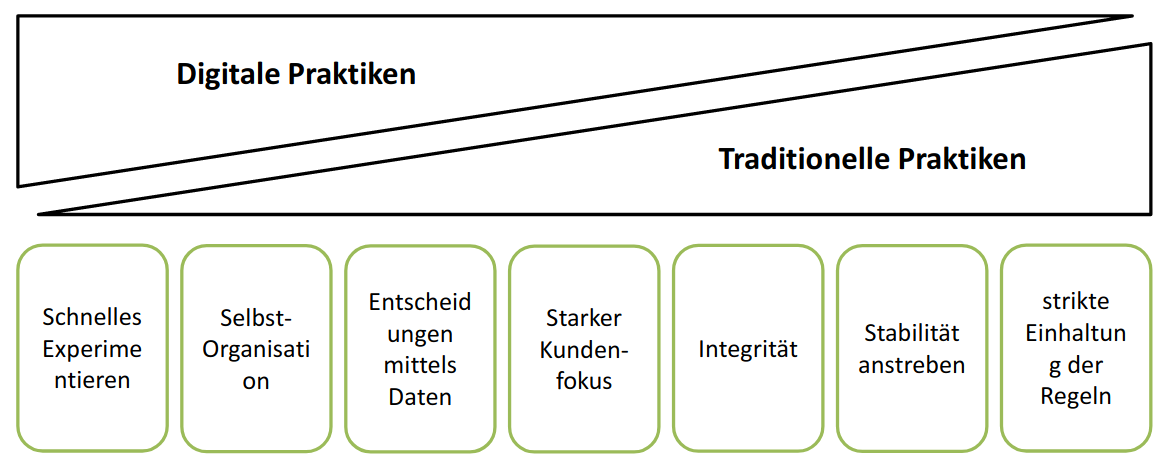
\includegraphics[scale=0.3]{altneu.png}
   
   \item \textbf{Digitale Transformation Leitfragen}
         \begin{itemize}
            \item Welche Technologien sind von zentraler Bedeutung für das Unternehmen?
            \item Mit welchen digitalen Angeboten und Prozessen werden zukünftig Erlöse generiert?
            \item Wie wird das Digitalgeschäft aufgebaut und geführt, welche strukturellen Anpassungen sind im Unternehmen erforderlich?
            \item Welche Investitionsmittel stehen zur Finanzierung des digitalen Transformationsvorhabens zur Verfügung?
         \end{itemize}

   \item \textbf{Transformationsprojekte als Enablerzur Veränderung der Organisation:}
   \item[] 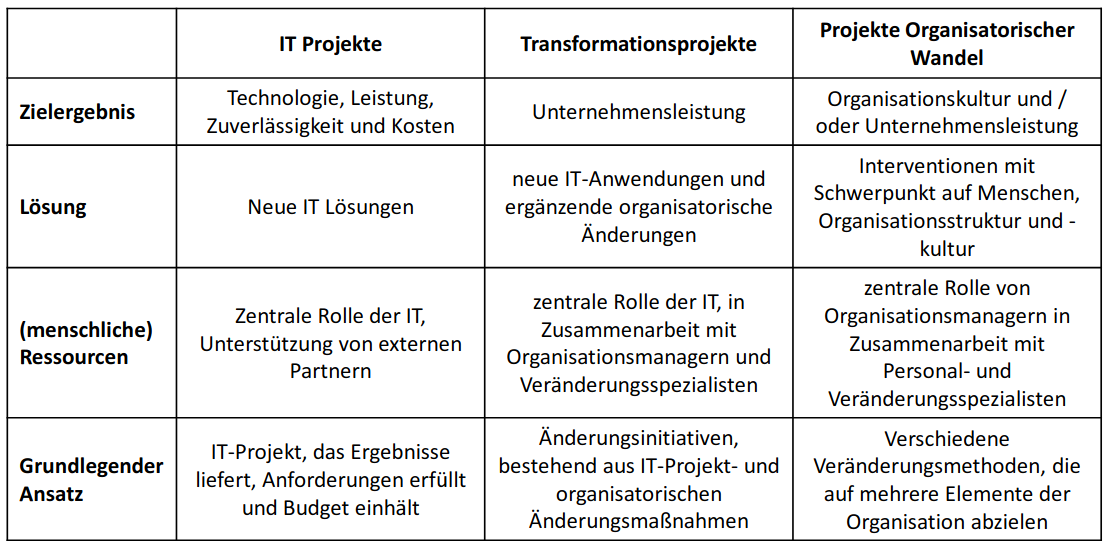
\includegraphics[scale=0.3]{ziele.png}
\end{itemize}


\newpage
\subsection{QUIZFRAGEN} %%%%%%%%%%%%%%%%%%%%%%%%%%%%%%%%%%%%%%%%%%%%%%%%%%%%%%%%%%%%%%%%%%%%%%%%%%%%%%%%%%%%%%%%%%%%%%%%%%%%%%%%%%%%%%
\begin{itemize}
   \item Übernahmen aufstrebender Konkurrenten als Reaktion auf neuartige / digitale Kon\-kur\-renz können für Unternehmen eine sinnvolle Alternative darstellen.
   \item Neuartige Geschäftsmodelle fokussieren sich im wesentlichen auf die Kundenerfahrung als Kernelement ihres Geschäftsmodells
   
   \item Bei \emph{Black-Hole} Investment Strategien ist der aggregierte negative \emph{Cassh Flow} in der Regel höher als bei Optionen-orientierte Investment Strategien.
   \item Bei der Black-Hole Investment Strategie werden alle Ressourcen auf ein einzelnes Investment allokiert.
   
   \item Der CDO arbeitet in der Regel eng mit dem Chief Executive Officer (CEO) zusammen.
   \item Ein CIO kümmert sich um die Effizienzsteigerung von Unternehmensprozessen und hat die Hauptaufgabe, die IT-Infrastruktur effizient zu managen.
   \item Der CIO ist für die IT-Struktur im Unternehmen verantwortlich, waehrend der CDO hauptsaechlich für die digitales und strategische Ausrichtung verantwortlich ist.
   
   \item Eine disruptive Innovation führt häufig zu einer völligen Umstrukturierung eines Marktes durch neuartige Geschäftsmodelle.
   
   \item Das Dilemma der Innovation (\textit{Innovator's Dilemma}) beschreibt den Zustand, dass etablierte Unternehmen weiter auf ihre traditionelle Geschäftspraxis setzen und so potenziell wichtige Technologien übersehen.
         Dies kann dazu führen, dass ehemalige Marktführer aus dem Markt gedrängt werden.
         
   \item Das S-Kurven Konzept als Instrument des strategischen Innovationsmanagements besagt, dass Technologien sich im Zeitverlauf in die Entstehungsphase, die Wachstumsphase, die Reifephase sowie die Phase der Alterung einteilen lassen.
         Darüber hinaus sind Basistechnologien im Markt bereits bekannt und etabliert, sodass sie keine bzw. kaum noch Wettbewerbsvorteile mit sich bringen.
         
   \item Eine Digitalkultur befähigt Mitarbeiter unternehmerisch zu denken, um neue Ge\-schäfts\-po\-ten\-zia\-le zu erkennen.
\end{itemize}

\end{document}